\documentclass[6008notes.tex]{subfiles}
\begin{document}
\graphicspath{ {images/viterbi/} }

\section{The Viterbi Algorithm}

Max-product or min-sum specialized to HMMs results in the Viterbi algorithm, proposed by MIT alum Andrew Viterbi back in 1967, which pre-dates both the forward-backward algorithm (1980) and the sum-product algorithm (1982). The Viterbi algorithm produces an MAP estimate for the sequence of hidden states given the observations of an HMM.

Let's work through an example. I have two coins, one fair and one biased, and I keep picking a coin and flipping it. You get to observe whether each flip was heads or tails, and from that information, you have to guess the sequence of coins that I used.

At first, I choose either the fair coin or the biased coin uniformly at random. I prefer not to switch between flips: that is, after each flip, my next flip will use the same coin with probability 3/4, and switch coins with probability 1/4. The fair coin is equally likely to be heads or tails, and the biased coin has probability 3/4 of coming up tails and probability 1/4 of coming up heads.

If you observe the sequence $HHTTT$ (where $H$ is heads and $T$ is tails), what's the most likely sequence of coins that I used?

We reuse notation from how we formulated HMM's when we presented the forward-backward algorithm. In particular, for this HMM with 5 hidden states, we define the following potentials:

\begin{eqnarray*}
\widetilde{\phi}_i(x_i)
&=&\begin{cases}
   p_{X_1}(x_1)p_{Y_1|X_1}(y_1|x_1) & \text{for }i=1, \\
   p_{Y_i|X_i}(y_i|x_i) & \text{for }i=2,\dots,5, \\
   \end{cases} \\
\psi(x_{i-1}, x_i)
&=&p_{X_i \mid X_{i-1}}(x_i \mid x_{i-1})
\quad\text{for }n=2,\dots,5.
\end{eqnarray*}

Thus, we have (importantly, observations $HHTTT$ have been folded into the node potentials!):

{\centering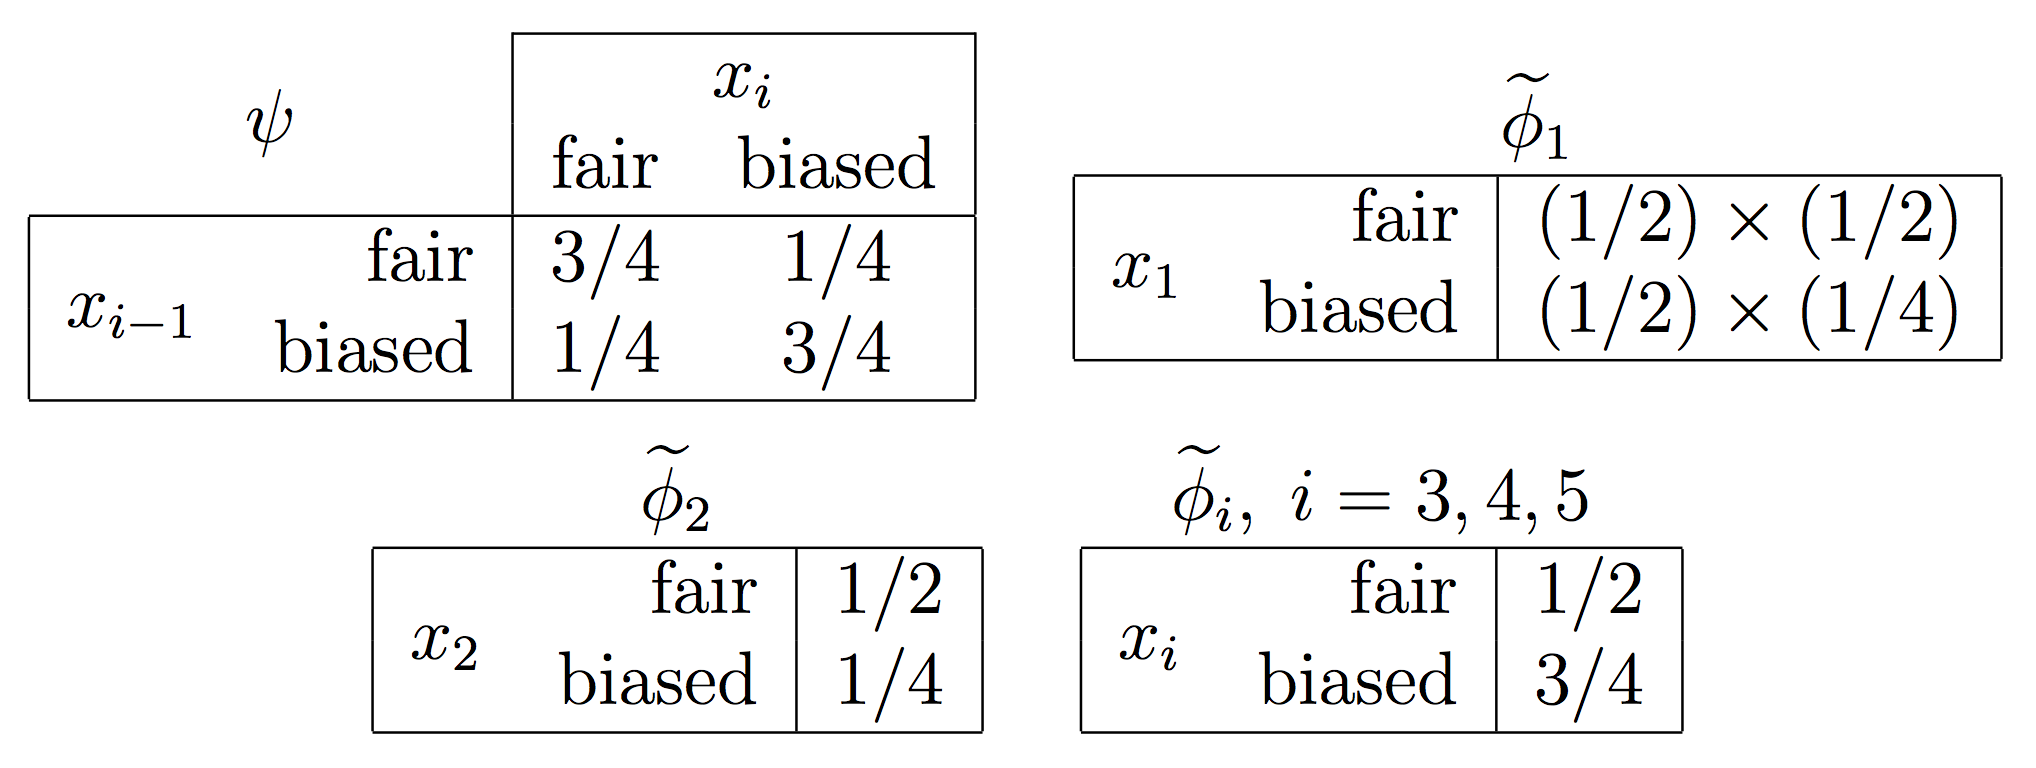
\includegraphics[scale=0.25]{images_sec-viterbi-example1} \par}

Defining $\gamma \triangleq \log _2(3) \approx 1.6$, we have:

{\centering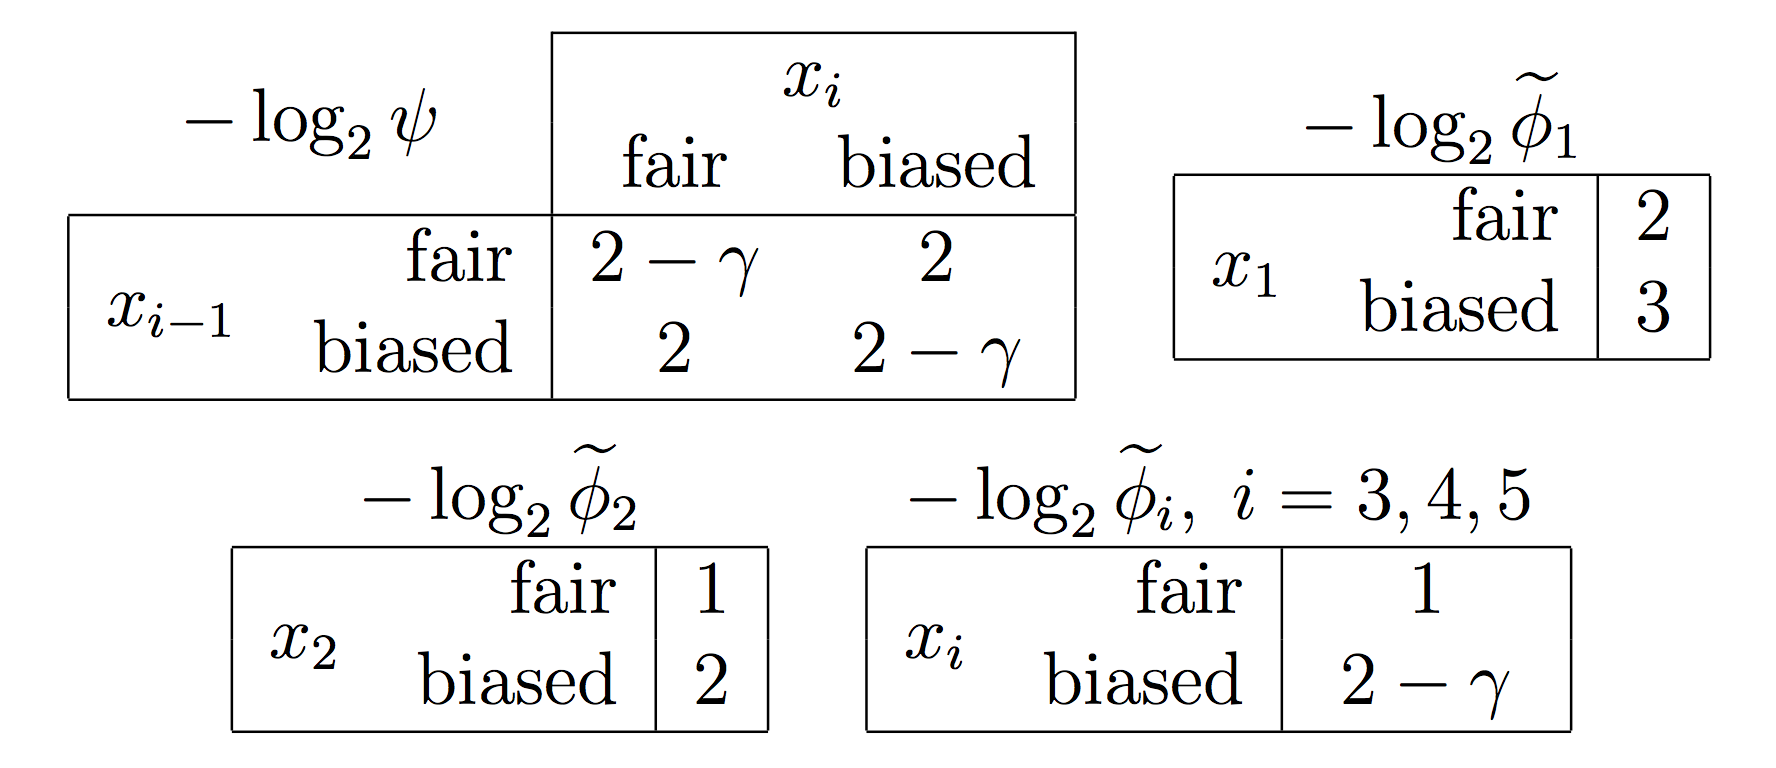
\includegraphics[scale=0.25]{images_sec-viterbi-example2} \par}

Below, we show what is called the \textit{trellis diagram} for this problem: note that while this diagram has nodes and edges, it is not a probabilistic graphical model in that the nodes do not correspond to random variables, and the nodes/edges aren't associated with potential tables, etc. Instead, the $i$-th column consists of all the possible states that $X_i$ can be, and the edges denote all possible transitions, so that a path going from left to right (a path in a trellis diagram can't go rightward and then leftward; it can only go rightward) corresponds to a specific possible sequence of states that $X_1,\dots ,X_ n$ can take on.

{\centering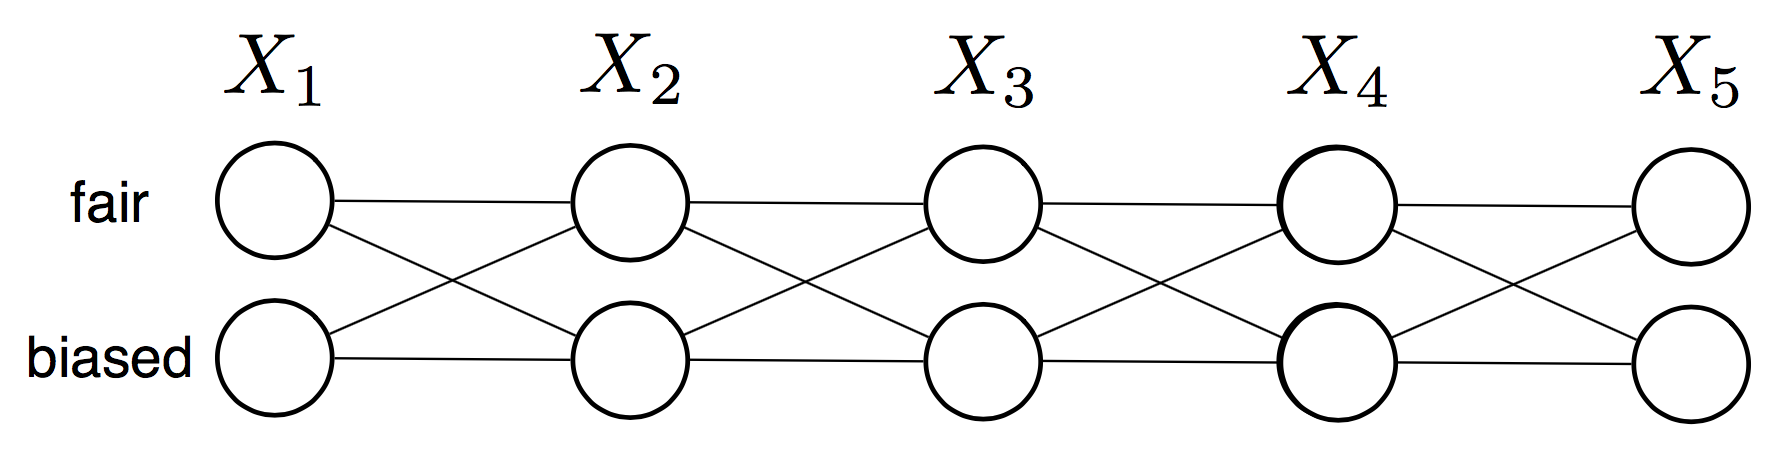
\includegraphics[scale=0.3]{images_sec-viterbi-trellis1}\\
The trellis diagram for our example \par}

We will see that the Viterbi algorithm just finds a path along this trellis.

For a length-$n$ HMM, the min-sum messages are

\begin{eqnarray*}
m_{1 \rightarrow 2}'(x_2)
&=& \min_{x_1}
      \left[
        -\log_2\widetilde{\phi}_1(x_1) - \log_2\psi(x_1,x_2)
      \right], \\
t_{2 \rightarrow 1}(x_2)
&=& \arg\min_{x_1}
      \left[
        -\log_2\widetilde{\phi}_1(x_1) - \log_2\psi(x_1,x_2)
      \right], \\
m_{(i-1) \rightarrow i}'(x_i)
&=& \min_{x_{i-1}}
      \left[
        -\log_2\widetilde{\phi}_{i-1}(x_{i-1})
        - \log_2\psi(x_{i-1},x_i)
        + m_{(i-2) \rightarrow (i-1)}'(x_{i-1})
      \right]
\qquad \text{for }i=3,\dots,n, \\
t_{i \rightarrow (i-1)}(x_i)
&=& \arg\min_{x_{i-1}}
      \left[
        -\log_2\widetilde{\phi}_{i-1}(x_{i-1})
        - \log_2\psi(x_{i-1},x_i)
        + m_{(i-2) \rightarrow (i-1)}'(x_{i-1})
      \right]
\qquad \text{for }i=3,\dots,n.
\end{eqnarray*}

Let's determine the messages for our length $n=5$ HMM.

We compute the first message:

\begin{eqnarray*}
m_{1\rightarrow 2}(\text{fair})
&=& \min_{x_1}
      \big[ -\log_2\widetilde\phi_1(x_1) - \log_2(\psi(x_1, \text{fair})) \big] \\
&=& \min
      \big\{
        \overbrace{-\log_2\widetilde\phi_1(\text{fair})
          - \log_2(\psi(\text{fair}, \text{fair}))}^{x_1 = \text{fair}}, \\
&&\qquad\;\;
        \underbrace{-\log_2\widetilde\phi_1(\text{biased})
          - \log_2(\psi(\text{biased}, \text{fair}))}_{x_1 = \text{biased}}
      \big\} \\
&=& \min
      \big\{
        \underbrace{2 + (2 - \gamma)}_{x_1 = \text{fair}},
        \underbrace{3 + 2}_{x_1 = \text{biased}}
      \big\} \\
&=& \min
      \big\{
        \underbrace{4 - \gamma}_{x_1 = \text{fair}},
        \underbrace{5}_{x_1 = \text{biased}}
      \big\} \\
&=& 4 - \gamma,
\end{eqnarray*}

where the $\arg \min$ is $x_1=fair$, so $t_{2\rightarrow 1}(\text {fair}) = \text {fair}$.

Next:

\begin{eqnarray*}
m_{1\rightarrow 2}(\text{biased})
&=& \min_{x_1}
      \big[ -\log_2\widetilde\phi_1(x_1) - \log_2(\psi(x_1, \text{biased})) \big] \\
&=& \min
      \big\{
        \overbrace{-\log_2\widetilde\phi_1(\text{fair})
          - \log_2(\psi(\text{fair}, \text{biased}))}^{x_1 = \text{fair}}, \\
&&\qquad\;\;
        \underbrace{-\log_2\widetilde\phi_1(\text{biased})
          - \log_2(\psi(\text{biased}, \text{biased}))}_{x_1 = \text{biased}}
      \big\} \\
&=& \min
      \big\{
        \underbrace{2 + 2}_{x_1 = \text{fair}},
        \underbrace{3 + (2 - \gamma)}_{x_1 = \text{biased}}
      \big\} \\
&=& \min
      \big\{
        \underbrace{4}_{x_1 = \text{fair}},
        \underbrace{5 - \gamma}_{x_1 = \text{biased}}
      \big\} \\
&=& 5 - \gamma,
\end{eqnarray*}

where the $\arg \min$ is $x_1=biased$, so $t_{2\rightarrow 1}(\text {biased}) = \text {biased}$.

Our message and traceback tables are then:

\begin{eqnarray*}
m_{1 \rightarrow 2}'(x_2)
&=& \begin{cases}
      4-\gamma & \text{if }x_2 = \text{fair} \\
      5-\gamma & \text{if }x_2 = \text{biased}
    \end{cases} \\
t_{2 \rightarrow 1}(x_2)
&=& \begin{cases}
      \text{fair} & \text{if }x_2 = \text{fair} \\
      \text{biased} & \text{if }x_2 = \text{biased}
    \end{cases}
\end{eqnarray*}

This traceback table tells us how to select x1 once we decide on x2. This is illustrated in the first-step trellis diagram below:

{\centering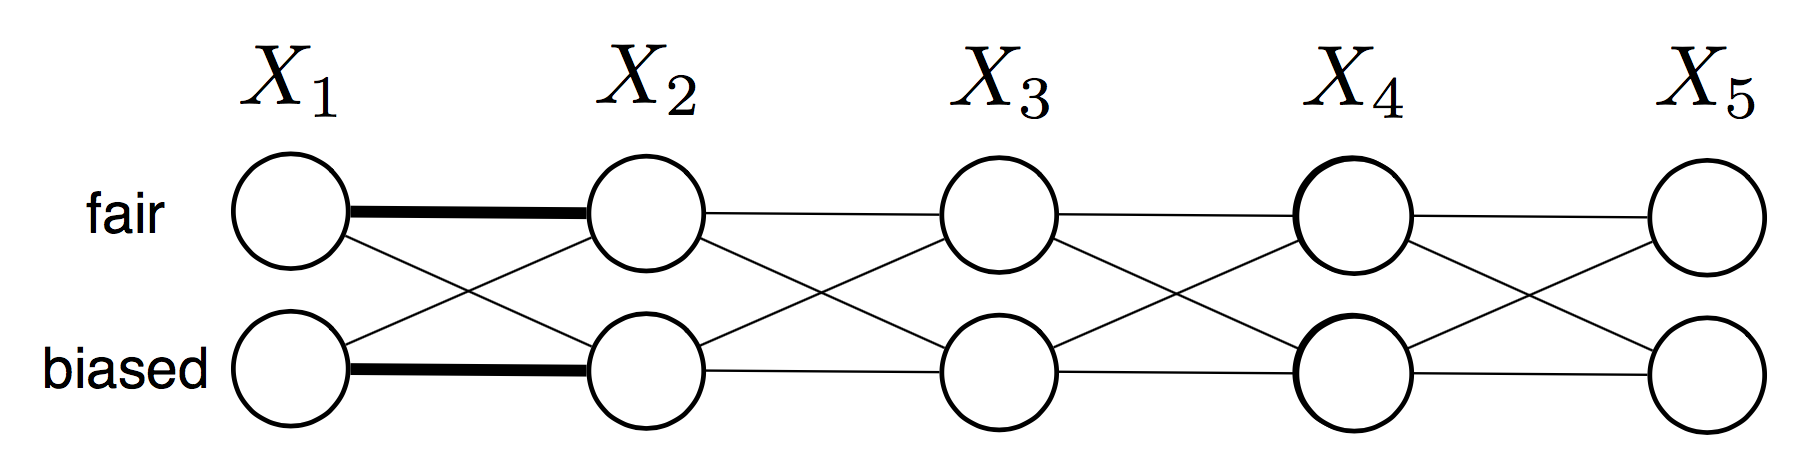
\includegraphics[scale=0.3]{images_sec-viterbi-trellis2}\\
The first traceback \par}

The second message is computed similarly:

\begin{eqnarray*}
m_{2\rightarrow 3}'(\text{fair})
&=& \min_{x_2}
      \big[ -\log_2\widetilde\phi_2(x_2) - \log_2(\psi(x_2, \text{fair}))
            + m_{1\rightarrow 2}'(x_2) \big] \\
&=& \min
      \big\{
        \overbrace{-\log_2\widetilde\phi_2(\text{fair})
          - \log_2(\psi(\text{fair}, \text{fair}))
          + m_{1\rightarrow 2}'(\text{fair})}^{x_2 = \text{fair}}, \\
&&\qquad\;\;
        \underbrace{-\log_2\widetilde\phi_2(\text{biased})
          - \log_2(\psi(\text{biased}, \text{fair}))
          + m_{1\rightarrow 2}'(\text{biased})}_{x_2 = \text{biased}}
      \big\} \\
&=& \min
      \big\{
        \underbrace{1 + (2 - \gamma) + (4 - \gamma)}_{x_2 = \text{fair}},
        \underbrace{2 + 2 + (5 - \gamma)}_{x_2 = \text{biased}}
      \big\} \\
&=& \min
      \big\{
        \underbrace{7 - 2\gamma}_{x_2 = \text{fair}},
        \underbrace{9 - \gamma}_{x_2 = \text{biased}}
      \big\} \\
&=& 7 - 2\gamma,
\end{eqnarray*}

where the $\arg \min$ is $x_2=fair$, so $t_{3\rightarrow 2}(\text {fair}) = \text {fair}$.

Next:

\begin{eqnarray*}
m_{2\rightarrow 3}'(\text{biased})
&=& \min_{x_2}
      \big[ -\log_2\widetilde\phi_2(x_2) - \log_2(\psi(x_2, \text{biased}))
            + m_{1\rightarrow 2}'(x_2) \big] \\
&=& \min
      \big\{
        \overbrace{-\log_2\widetilde\phi_2(\text{fair})
          - \log_2(\psi(\text{fair}, \text{biased}))
          + m_{1\rightarrow 2}'(\text{fair})}^{x_2 = \text{fair}}, \\
&&\qquad\;\;
        \underbrace{-\log_2\widetilde\phi_2(\text{biased})
          - \log_2(\psi(\text{biased}, \text{biased}))
          + m_{1\rightarrow 2}'(\text{biased})}_{x_2 = \text{biased}}
      \big\} \\
&=& \min
      \big\{
        \underbrace{1 + 2 + (4 - \gamma)}_{x_2 = \text{fair}},
        \underbrace{2 + (2 - \gamma) + (5 - \gamma)}_{x_2 = \text{biased}}
      \big\} \\
&=& \min
      \big\{
        \underbrace{7 - \gamma}_{x_2 = \text{fair}},
        \underbrace{9 - 2\gamma}_{x_2 = \text{biased}}
      \big\} \\
&=& 7 - \gamma,
\end{eqnarray*}

where the $\arg \min$ is $x_2=fair$, so $t_{3\rightarrow 2}(\text {biased}) = \text {fair}$.

Our message and traceback tables are then:

\begin{eqnarray*}
m_{2 \rightarrow 3}'(x_3)
&=& \begin{cases}
      7-2\gamma & \text{if }x_3 = \text{fair} \\
      7-\gamma & \text{if }x_3 = \text{biased}
    \end{cases} \\
t_{3 \rightarrow 2}(x_3)
&=& \begin{cases}
      \text{fair} & \text{if }x_3 = \text{fair} \\
      \text{fair} & \text{if }x_3 = \text{biased}
    \end{cases}
\end{eqnarray*}

The traceback is illustrated below:

{\centering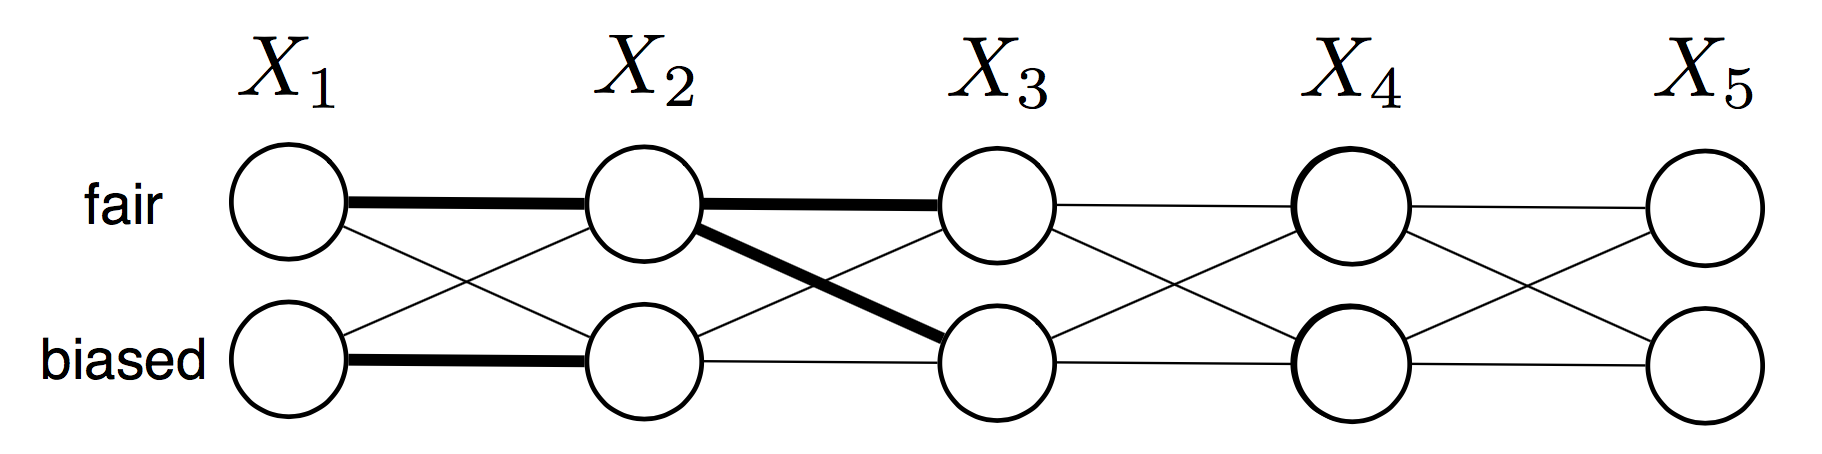
\includegraphics[scale=0.3]{images_sec-viterbi-trellis3}\\
The second traceback \par}

We see that after observing wo heads in a row, we will eventually pick $x_2=$ fair no matter what $x_3$ is.

Make sure that you can also compute these messages! The rest of the message and traceback tables are as follows:

\begin{eqnarray*}
m_{3 \rightarrow 4}'(x_4)
&=& \begin{cases}
      10-3\gamma & \text{if }x_4 = \text{fair} \\
      11-3\gamma & \text{if }x_4 = \text{biased}
    \end{cases} \\
t_{4 \rightarrow 3}(x_4)
&=& \begin{cases}
      \text{fair} & \text{if }x_4 = \text{fair} \\
      \text{biased} & \text{if }x_4 = \text{biased}
    \end{cases} \\
m_{4 \rightarrow 5}'(x_5)
&=& \begin{cases}
      13-4\gamma & \text{if }x_5 = \text{fair} \\
      15-5\gamma & \text{if }x_5 = \text{biased}
    \end{cases} \\
t_{5 \rightarrow 4}(x_5)
&=& \begin{cases}
      \text{fair} & \text{if }x_5 = \text{fair} \\
      \text{biased} & \text{if }x_5 = \text{biased}
    \end{cases} \\
\end{eqnarray*}

The traceback is illustrated below:

{\centering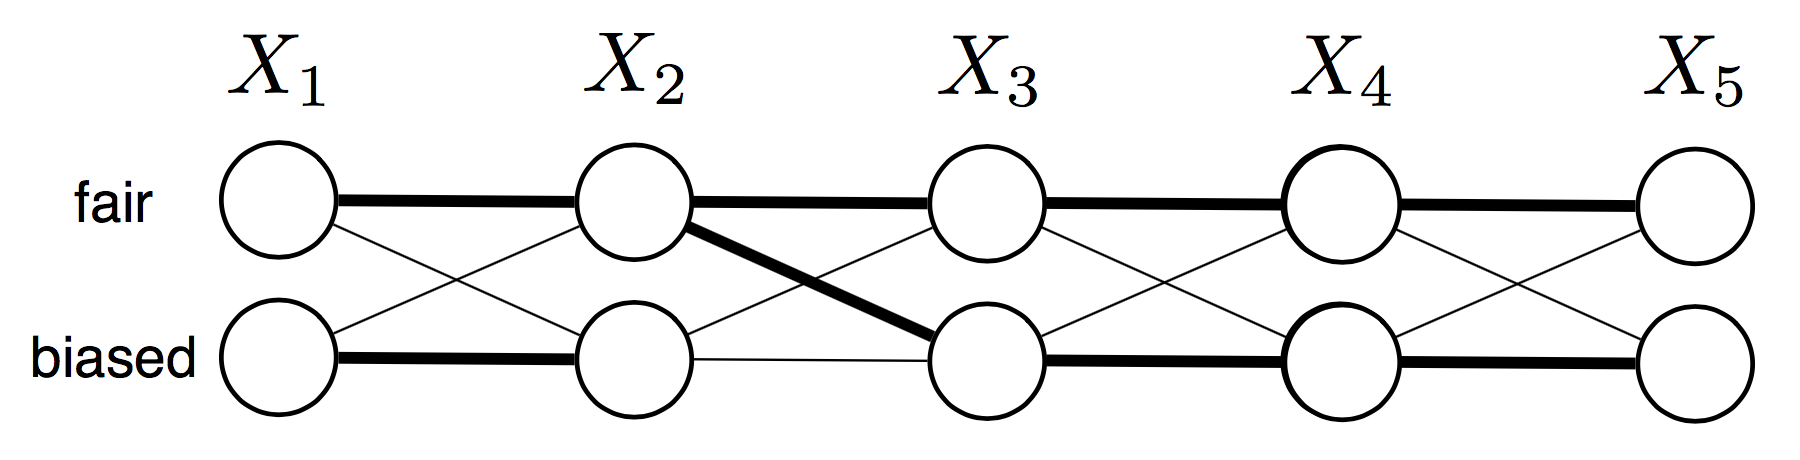
\includegraphics[scale=0.3]{images_sec-viterbi-trellis5}\\
The final traceback \par}

Finally, we can compute the most likely value for $X_5$:

\begin{eqnarray*}
\hat{x}_5 &=&
\arg\min \Big( \underbrace{1 + (13 - 4\gamma) }_{x_5 = \text{fair}} , \underbrace{(2-\gamma) + (15-5\gamma)}_{x_5 = \text{biased}} \Big) 
    = \text{biased}
\end{eqnarray*}

We can see from the trellis diagram that as soon as we decide on a value for $X_5$, we just have to follow our ``trail of breadcrumbs'' from the traceback messages to get the path highlighted below:

{\centering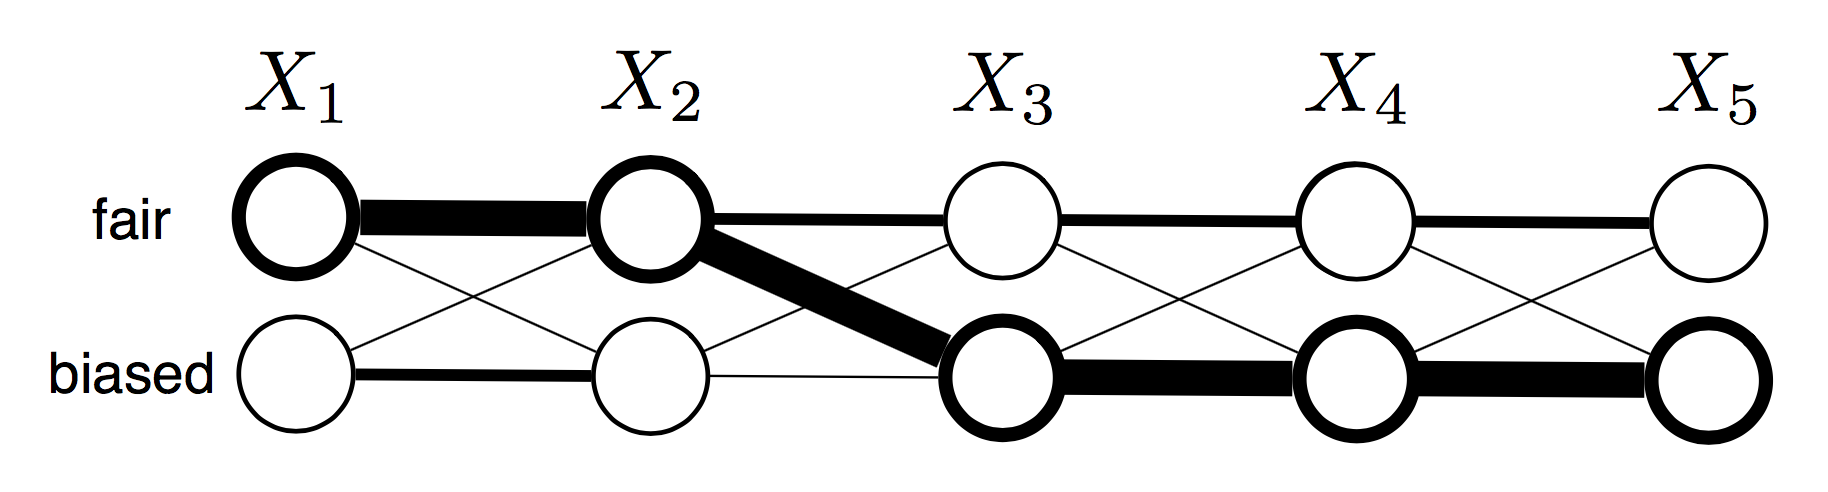
\includegraphics[scale=0.3]{images_sec-viterbi-trellis6}\\
The result of the Viterbi algorithm \par}

We can do the same thing with the traceback messages:

\begin{eqnarray*}
\hat{x}_4 &=& t_{5 \rightarrow 4}(\hat{x}_5) 
          = \text{biased} \\
\hat{x}_3 &=& t_{4 \rightarrow 3}(\hat{x}_4) 
          = \text{biased} \\
\hat{x}_2 &=& t_{3 \rightarrow 2}(\hat{x}_3) 
          = \text{fair} \\
\hat{x}_1 &=& t_{2 \rightarrow 1}(\hat{x}_2) 
          = \text{fair} \\
\end{eqnarray*}

We conclude that the MAP estimate for the sequence of hidden states given observed sequence $HHTTT$ is ``fair, fair, biased, biased, biased''.



\end{document}
